\documentclass[]{article}
\usepackage{graphicx}
\usepackage{subfigure}
\usepackage{epstopdf}
\usepackage{caption}
\usepackage{float}
\usepackage{amsmath,amssymb,amsfonts}
\usepackage{listings}
\usepackage{newlfont}
\usepackage{algorithm}
\usepackage{algorithmic}

\begin{document}

\title{Nonuniqueness of Dantzig solution path}
\author{Cheng Tai}
\date{}
\maketitle

\section{Experiments}
\textbf{Set up}
X = [1 1 2 1; 1 0 1 2; 0 1 1 0];
Y = [9.1 7.2 2.8]
$\beta$ = [2 0 3 1];

\begin{figure}[htp!]\centering 
\begin{tabular}{cc}
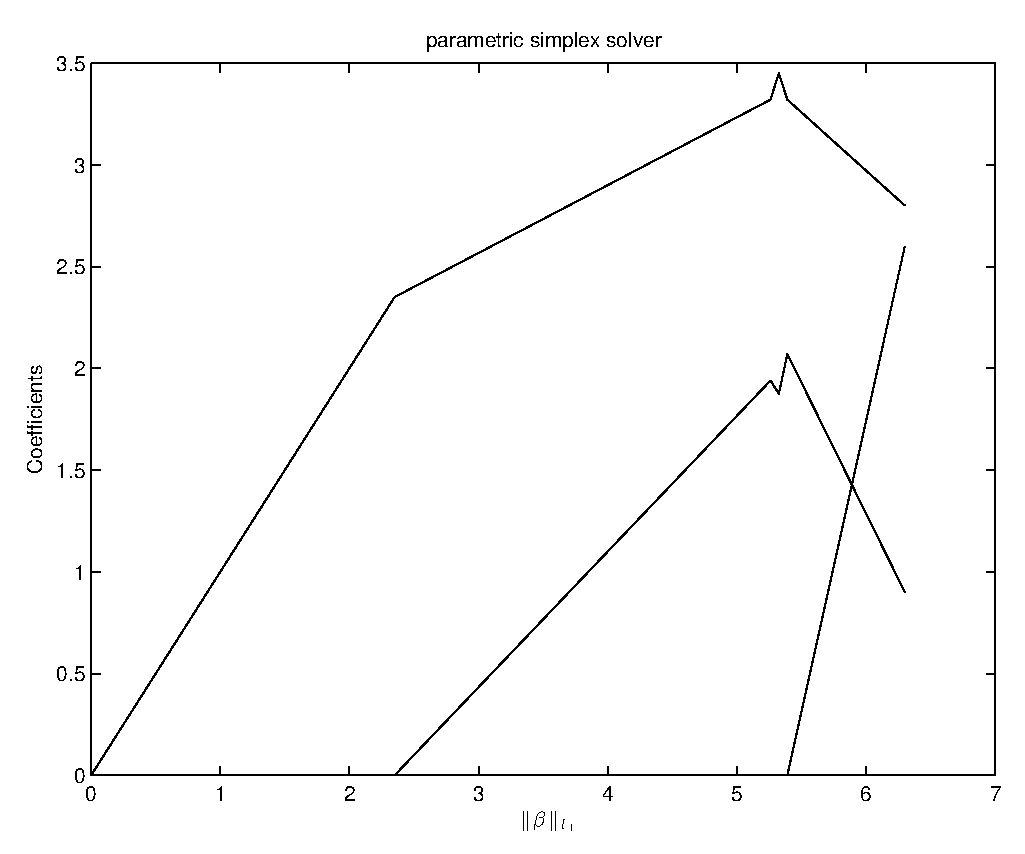
\includegraphics[width=0.5 \textwidth]{ps1.eps}& 
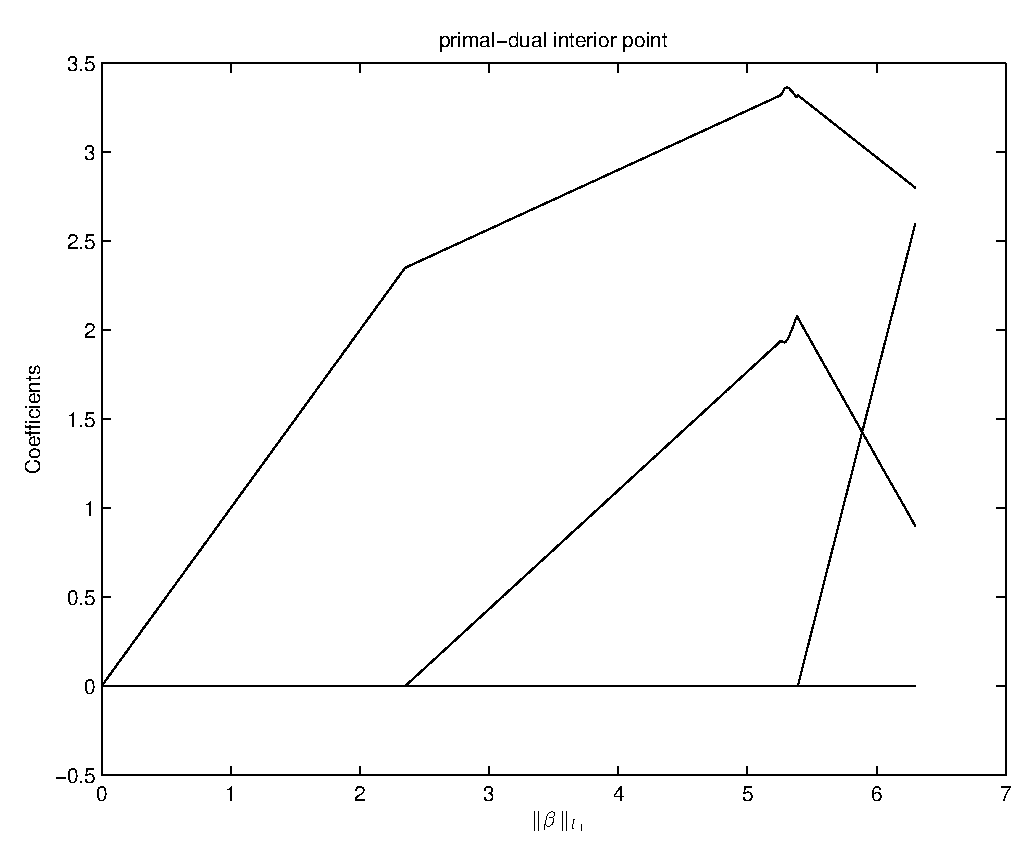
\includegraphics[width=0.5 \textwidth]{pd1.eps}\\
(a) & (b)\\
\end{tabular}
\caption{Solution path: (a) produced by parametric simplex algorithm. (b) produced by primal-dual interior point algorithm}
\end{figure}
\begin{figure}[htp!]\centering 
\begin{tabular}{cc}
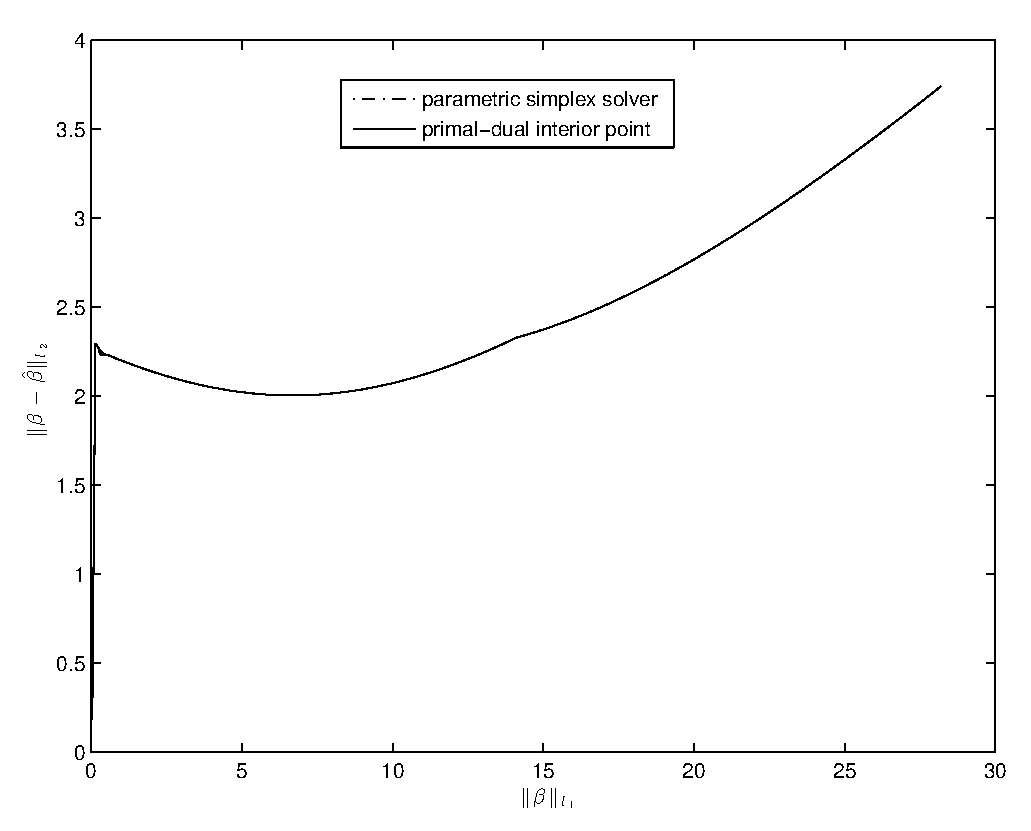
\includegraphics[width=0.5 \textwidth]{compare1.eps}& 
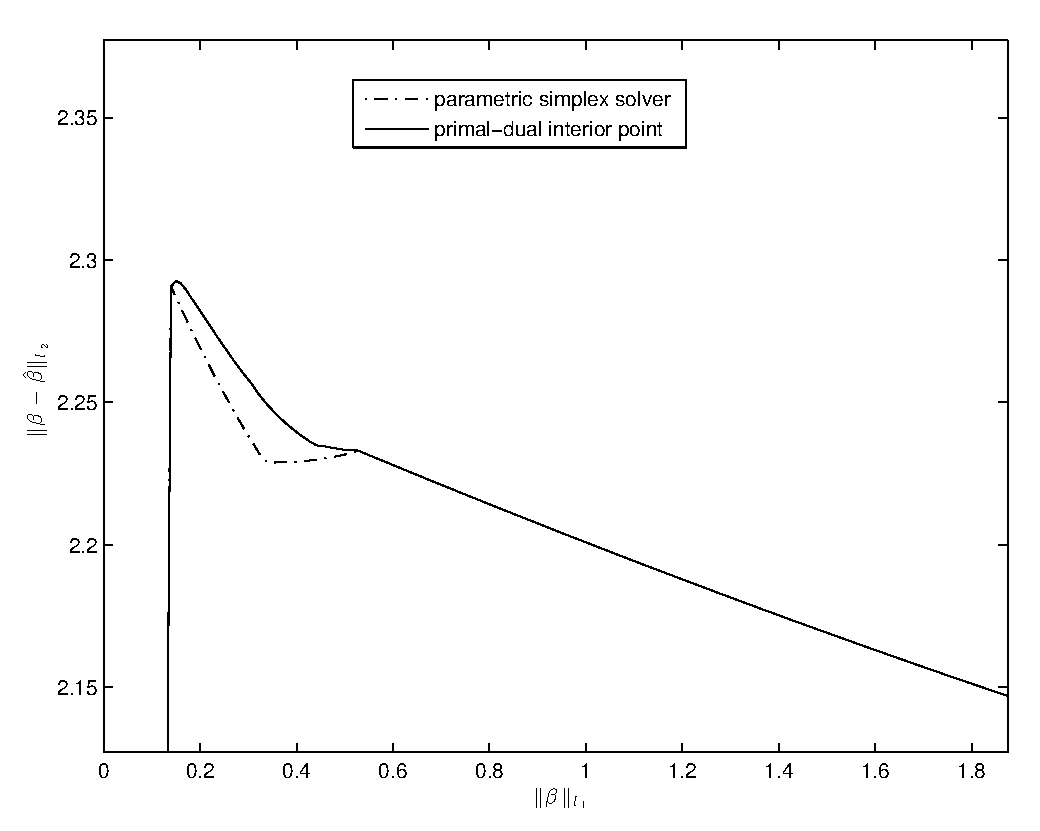
\includegraphics[width=0.5 \textwidth]{compare1_1.eps}\\
(a) & (b)\\
\end{tabular}
\caption{Solution path: (a) Error measured by $\|\beta-\hat\beta\|_{l_2}$, (b) zoom in}
\end{figure}

$\lambda  = 0.3$, x1 = [0 0 3.4333 1.900], xp= [0 0 3.3505 1.9828]; both have l1 norm 5.3333, and 
for x1, $X'(Y-X*\hat\beta)=[ 0.3 -0.3 0 0.2667]$, for xp $X'(Y-X*\hat\beta) = [0.3 00.1344 0.1656 0.1839]$.
However, their l1 error is the same.

\begin{figure}[htp!]\centering 

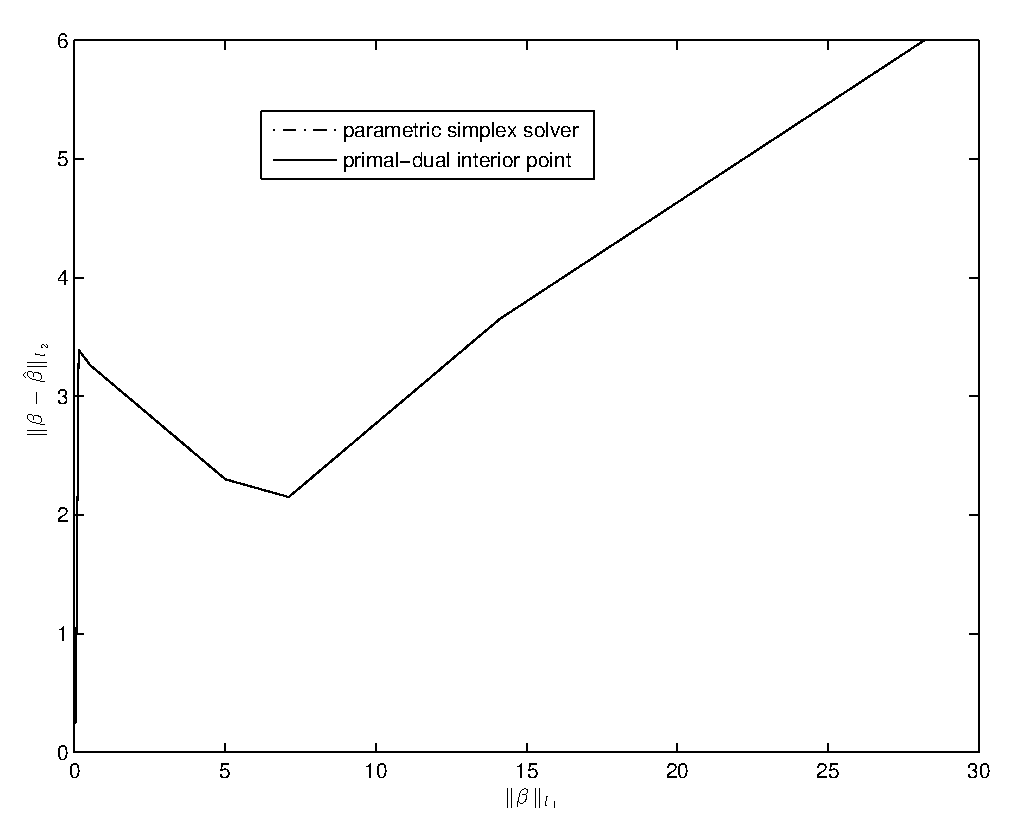
\includegraphics[width=0.5 \textwidth]{compare12.eps}\\

\caption{Solution path: Error measured by $\|\beta-\hat\beta\|_{l_1}$}
\end{figure}


















\end{document}